\documentclass{article}

%encoding
%--------------------------------------
\usepackage[utf8]{inputenc}
\usepackage[T1]{fontenc}
%----------------------------

%fonts
%--------------------------------------
%---------------
% \setromanfont{Times New Roman}
% \setsansfont{Arial}
% \setmonofont[Color={0019D4}]{Courier New}
%
\usepackage{libertine}
\usepackage{beramono}

%units
%--------------------------------------
\usepackage{siunitx}

%drawing
%------------------------------------
\usepackage{tikz} % To generate the plot from csv
\usepackage{pgfplots}
\usepackage{pgfplotstable}

\usetikzlibrary{datavisualization}
\pgfplotsset{compat=newest} % Allows to place the legend below plot
\usepgfplotslibrary{units} % Allows to enter the units nicely

\sisetup{
  round-mode          = places,
  round-precision     = 2,
}

\begin{document}

\begin{figure}
  \begin{center}

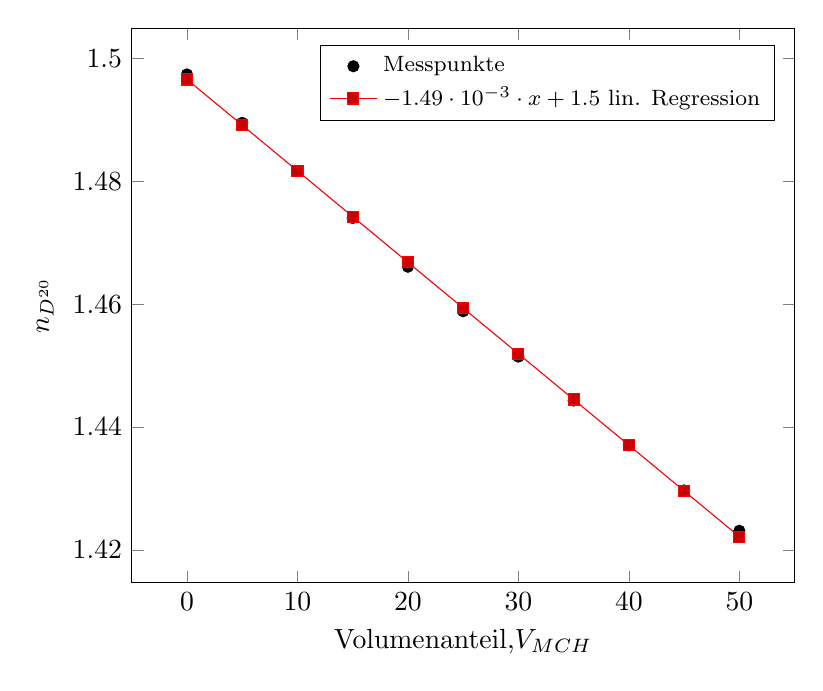
\begin{tikzpicture}
    \pgfplotsset{width=10cm,
        compat=1.3,
        legend style={font=\footnotesize}}
    \begin{axis}[
    xlabel={Volumenanteil,$V_{MCH}$},
    ylabel={$n_{D^{20}}$},
    legend cell align=left,
    legend pos=north east]
    \addplot[only marks] table{
        0 1.49736
        5 1.48948
        10 1.48163
        15 1.47401
        20 1.46608
        25 1.45884
        30 1.45146
        35 1.44432
        40 1.43702
        45 1.42969
        50 1.42312
    };
    \addplot table[y={create col/linear regression={y=Y}}]{
        X Y
        0 1.49736
        5 1.48948
        10 1.48163
        15 1.47401
        20 1.46608
        25 1.45884
        30 1.45146
        35 1.44432
        40 1.43702
        45 1.42969
        50 1.42312
};

    \addlegendentry{Messpunkte}
    \addlegendentry{%
        $\pgfmathprintnumber{\pgfplotstableregressiona} \cdot x
        \pgfmathprintnumber[print sign]{\pgfplotstableregressionb}$ lin. Regression} %
    \end{axis}
    \end{tikzpicture}
\end{center}
\end{figure}

\begin{figure}
  \begin{center}

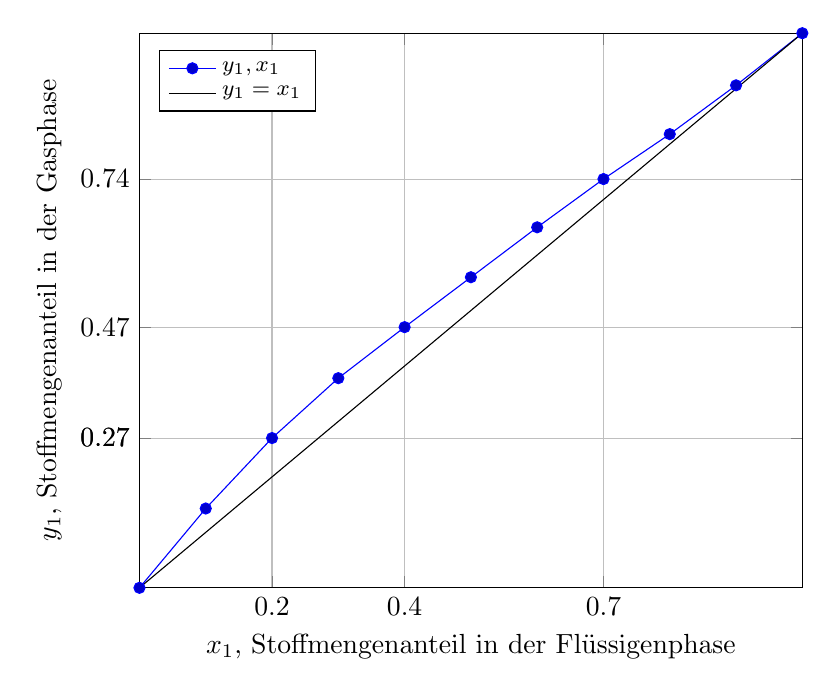
\begin{tikzpicture}
    \pgfplotsset{width=10cm,
        compat=1.3,
        legend style={font=\footnotesize}}

    \begin{axis}[
    xmin=0, xmax=1,
    ymin=0, ymax=1,
    xlabel={$x_1$, Stoffmengenanteil in der Flüssigenphase},
    ylabel={$y_1$, Stoffmengenanteil in der Gasphase},
    ytick={0.270, 0.270, 0.470, 0.737},
    xtick={0.2, 0.4, 0.7},
    ymajorgrids=true,
    xmajorgrids=true,
    legend cell align=left,
    legend pos=north west]
    \addplot table{
        0.00 0.000
        0.10 0.143
        0.20 0.270
        0.30 0.378
        0.40 0.470
        0.50 0.560
        0.60 0.650
        0.70 0.737
        0.80 0.818
        0.90 0.906
        1.00 1.000
    };
    \addplot [domain=0:1, color = black] {x} ;
    \addlegendentry{$y_1,x_1$}
    \addlegendentry{$y_1=x_1$}
    \end{axis}


    \end{tikzpicture}
\end{center}
\caption{Siedediagramm}
\end{figure}

\tikz \datavisualization [
scientific axes, visualize as line,
x axis={ticks={ minor steps between steps=3},
label=Siedediagramm}]
data {
x, y
   0.00, 0.000
        0.10, 0.143
        0.20, 0.270
        0.30, 0.378
        0.40, 0.470
        0.50, 0.560
        0.60, 0.650
        0.70, 0.737
        0.80, 0.818
        0.90, 0.906
        1.00, 1.000
};

\end{document}